\documentclass[11pt,letterpaper]{article}
\usepackage[T1]{fontenc}
\usepackage[utf8]{inputenc}
\usepackage[margin=0.91in,headheight=15pt]{geometry}
\usepackage{mathpazo}
\usepackage{amsmath,amssymb,amsthm}
\usepackage{graphicx,booktabs,array}
\usepackage[font=small,labelfont=bf]{caption}
\usepackage[section]{placeins}
\usepackage{microtype,parskip}
\usepackage{xcolor}
\usepackage{fancyhdr}
\usepackage{enumitem}
\usepackage[numbers,sort&compress]{natbib}
\usepackage{url}
\usepackage{hyperref}
\definecolor{ink}{HTML}{243443}
\definecolor{teal}{HTML}{087F8C}
\hypersetup{colorlinks=true,linkcolor=teal,citecolor=teal,urlcolor=teal,
 pdftitle={3D Labyrinth: A Two-Thirds-Air, One-Third-Bedrock Random Voxel Maze},
 pdfauthor={Kaoru Aguilera Katayama}}
\setlength{\parskip}{5pt plus 1pt}
\setlength{\parindent}{0pt}
\clubpenalty=10000
\widowpenalty=10000
\brokenpenalty=10000
\setlength{\textfloatsep}{14pt plus 2pt minus 2pt}
\setlength{\intextsep}{12pt plus 2pt minus 2pt}
\setcounter{topnumber}{3}
\renewcommand{\topfraction}{.9}
\renewcommand{\textfraction}{.08}
\renewcommand{\floatpagefraction}{.75}
\pagestyle{fancy}
\fancyhf{}
\fancyhead[L]{\small\textsc{3D Labyrinth}}
\fancyhead[R]{\small Kaoru Aguilera Katayama}
\fancyfoot[C]{\small\thepage}
\renewcommand{\headrulewidth}{.3pt}
\newtheorem{proposition}{Proposition}
\newcommand{\E}{\mathbb{E}}
\newcommand{\Prob}{\mathbb{P}}
\newcommand{\Var}{\operatorname{Var}}
\newcommand{\Cov}{\operatorname{Cov}}
\newcommand{\ind}{\mathbf{1}}
\newcommand{\G}{G_{L,p}}
\newcommand{\Hh}{H_{L,p}}
\newcommand{\air}{\mathrm{air}}
\newcommand{\bed}{\mathrm{bedrock}}
\newcommand{\smallhead}[1]{\medskip\noindent\textbf{#1}\quad}

\begin{document}
\thispagestyle{plain}
\begin{center}
 {\Large\bfseries\color{ink} 3D Labyrinth}\\[5pt]
 {\large A Two-Thirds-Air, One-Third-Bedrock Random Voxel Maze}\\[13pt]
 {\normalsize Kaoru Aguilera Katayama}\\[3pt]
 {\small October 6, 2026; repository edition: October 7, 2026}
\end{center}
\vspace{3pt}
\begin{abstract}
A simple Minecraft construction replaces the voxels of a cube independently
with air with probability $2/3$ and bedrock with probability $1/3$.
The resulting object is a three-dimensional labyrinth whose passages emerge
from random placement rather than from a prescribed corridor network.
We formalize this construction as finite site percolation and distinguish
connectivity of single air voxels from collision-free translation of an upright
two-voxel body. Exact formulas describe occupancy, adjacency, and the dependence
introduced by head clearance. A reproducible experiment uses 9,300 random cubes
to study face-to-face crossings, useful entrances, connected components, and
shortest routes. At the proposed density, all 300 cubes of each tested side
length $16$, $32$, and $64$ admit a crossing in both movement models.
At side length $64$, mean shortest-route length from a randomly selected open
entry is $1.207$ times the cube width in the one-voxel model and $1.604$ times
the width in the upright-body model, conditional on reaching the opposite face.
These results support the construction as a highly connected exploration maze
with nontrivial detours. We also describe how entrance selection and an explicit
movement rule turn the random volume into a well-defined playable challenge.
\end{abstract}
\noindent\textbf{Keywords:} random voxel maze; site percolation; procedural generation;
Minecraft; configuration space; pathfinding.

\section{Introduction}
The starting point is an experiment conceived and built by the author during a
Minecraft livestream: select a cube, fill it randomly with two parts air and one
part bedrock, and explore the passages that appear. The player must discover
where entry and movement are possible. Unlike a maze assembled from a sequence
of carved corridors, the complete three-dimensional volume is randomized at
once. Tunnels, small chambers, loops, blocked openings, and changes in elevation
are consequences of the same local rule.

This paper develops a mathematical and computational account of that design.
The independent random-volume model is an instance of site percolation on the
simple-cubic lattice. The central design question is how this familiar model
behaves when interpreted as a navigable voxel labyrinth, particularly at the
author's chosen air probability $p=2/3$.

Three distinctions organize the analysis. First, a $2{:}1$ random weighting
specifies an expected composition, whereas an exactly fixed composition is a
different sampling rule. Second, a connected sequence of air cells may be too
small for a body with height. Third, a cube can contain a crossing even though
a particular opening leads to a component that does not reach the exit.
These distinctions lead to measurable properties of the construction without
requiring Minecraft to run the experiments.

The contribution is a reproducible design study: a precise generator, two
movement graphs, elementary analytic predictions, finite-size experiments, and
rules for converting random geometry into an entry-to-exit objective.
The author's report of enjoyable play motivates the study; the numerical
experiments measure geometry and graph navigation, rather than player enjoyment
or completion times.

\section{Random-voxel construction}
\subsection{The two-to-one rule}
For an integer $L\geq 3$, let $\Lambda_L=\{0,\ldots,L-1\}^{3}$ be a cube with
$N=L^3$ unit voxels. Coordinates are $(x,y,z)$; throughout the mathematical
model, $z$ denotes height. This is a coordinate convention, with a relabeling
needed when a game uses another vertical axis.
For each $v\in\Lambda_L$, sample an independent variable $X_v$ with
\begin{equation}
 \Prob(X_v=1)=p,\qquad \Prob(X_v=0)=1-p.
 \label{eq:generator}
\end{equation}
The value $1$ denotes air and $0$ denotes an impassable bedrock voxel.
The proposed labyrinth uses $p=2/3$. Bedrock is treated as a fixed obstacle:
changing blocks is outside the navigation rules, irrespective of the game mode.

WorldEdit documents comma-separated random patterns and relative weights
\citep{worldedit}. A direct expression of the intended $2{:}1$ rule is
\begin{center}
\fbox{\texttt{//set 2\%air,1\%bedrock}}
\end{center}
after selecting the desired cube. The percentage signs in this pattern specify
relative weights, so the total weight is three. The author's description of two
air entries and one bedrock entry expresses the same intended mixture.
Our experiments use an explicitly independent pseudorandom generator; they do
not assert bit-for-bit equivalence with a particular WorldEdit implementation.

Let $A=\sum_v X_v$. Then $A\sim\operatorname{Binomial}(L^3,p)$,
$\E[A]=pL^3$, and $\Var(A)=L^3p(1-p)$. Consequently,
\begin{equation}
 \E\!\left[\frac{A}{L^3}\right]=\frac23,
 \qquad
 \operatorname{sd}\!\left(\frac{A}{L^3}\right)
 =\sqrt{\frac{2}{9L^3}}
 \quad\text{at }p=\frac23.
 \label{eq:fluctuations}
\end{equation}
For $L=64$, this standard deviation is approximately $0.000921$ as a fraction,
or $0.0921$ percentage points. Thus the observed ratio concentrates around the
target as the cube grows.

\subsection{An exact-composition variant}
If an exact count is required, choose $K=\lfloor 2L^3/3\rfloor$ air positions
uniformly without replacement and fill the remaining cells with bedrock.
For distinct $u,v$, this ensemble has $\Prob(X_v=1)=K/N$ and
$\Prob(X_u=X_v=1)=K(K-1)/[N(N-1)]$. The indicators are no longer independent.
An exactly two-thirds fraction is possible when $3$ divides $L^3$; otherwise
rounding is unavoidable. All experiments below use
Equation~\eqref{eq:generator}, not this fixed-count variant.

\section{From empty cells to movement graphs}
\subsection{One-voxel navigation}
Define the undirected graph $\G=(V_G,E_G)$ by
$V_G=\{v\in\Lambda_L:X_v=1\}$ and
$E_G=\{\{u,v\}:u,v\in V_G,\ \lVert u-v\rVert_1=1\}$.
Only face-sharing voxels are adjacent; touching at an edge or corner does not
create a passage. This graph represents a lattice agent occupying one voxel
and moving along any of the six coordinate directions.
It includes vertical motion and is a geometric navigation model, rather than
a gravity-based walking model.

The entrance face is $F_0=\{v:x=0\}$ and the exit face is
$F_1=\{v:x=L-1\}$. A crossing is a graph path connecting admissible vertices
on these two faces. All paths remain inside the cube. There are no periodic
boundaries and no exterior route that can bypass the obstacles.

\subsection{Upright two-voxel clearance}
A player-sized passage requires more than one empty cell. To capture the effect
of height without reproducing game physics, consider a rigid, axis-aligned
$1\times1\times2$ body. Its lower voxel is anchored at
$v=(x,y,z)\in\Lambda_L^{(2)}=\{0,\ldots,L-1\}^{2}\times\{0,\ldots,L-2\}$.
An anchor is admissible when
\begin{equation}
 Y_v=X_vX_{v+e_z}=1.
 \label{eq:clearance}
\end{equation}
The graph $\Hh$ connects admissible anchors at Manhattan distance one.
The body remains upright and translates by one voxel per edge.
For these axis-aligned unit translations, the swept body lies in the union of
the endpoint cells: horizontal motion requires four air voxels and vertical
motion requires three. Hence these edges are collision-free under the stated
voxel-body convention. This is a discrete configuration-space construction
\citep{lavalle2006}.

\begin{figure}[htbp]
\centering
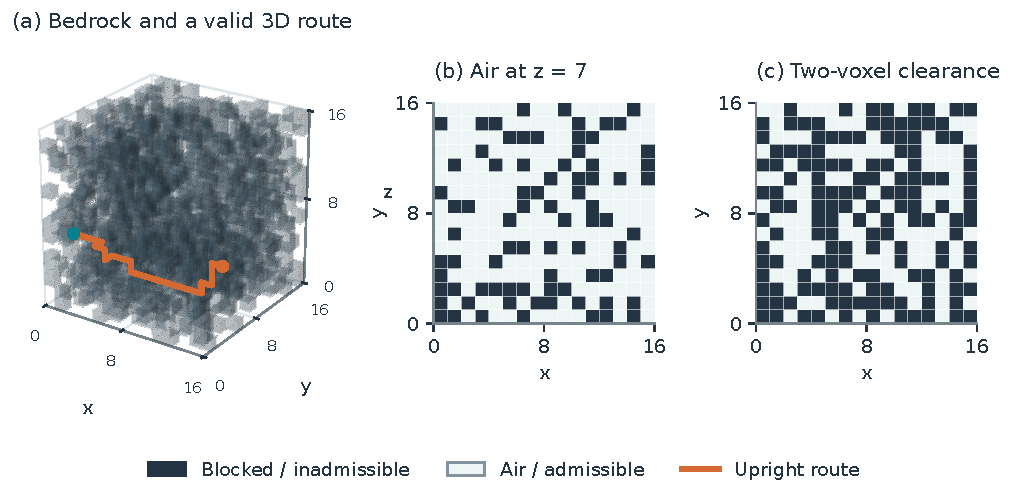
\includegraphics[width=\linewidth]{figures/01_geometry.pdf}
\caption{One reproducible $16^3$ realization at $p=2/3$.
(a) Bedrock with a corner omitted from the drawing and an upright-body path
overlaid for visibility; no obstacles were removed for pathfinding.
The route has 22 edges, versus a width of $L-1=15$.
(b) Air in the horizontal layer $z=7$.
(c) Admissible lower-body positions at $z=7$, requiring air at both $z=7$ and
$z=8$. Pale cells are available; dark cells are blocked in the relevant model.
The illustration uses a separate, specified seed and is outside the 9,300-cube
statistical sample.}
\label{fig:geometry}
\end{figure}

The admissible-anchor density is $\E[Y_v]=p^2=4/9$ at the proposed setting.
However, adjacent anchors in a vertical column share a required air voxel:
\begin{equation}
 \Cov(Y_v,Y_{v+e_z})=p^3-p^4=p^3(1-p)>0
 \quad (0<p<1).
 \label{eq:dependence}
\end{equation}
Thus $H$ is a dependent occupancy model. Substituting $p^2$ into an independent
site-percolation threshold would ignore this dependence.
For an interior admissible anchor, expected degree is $4p^2+2p$, equal to
$28/9$ at $p=2/3$.

Both graphs allow unrestricted vertical translation. Standing, jumping,
falling, crawling, and actual collision-box dimensions require an additional
movement specification. For example, an interior supported standing position
under the same two-voxel approximation satisfies
$X_vX_{v+e_z}(1-X_{v-e_z})=1$, an event of probability
$p^2(1-p)=4/27$. This is a local availability calculation, not a test of
survival-mode reachability. The experiments therefore directly address abstract
flight-like navigation with collision clearance.

\section{Elementary properties of the labyrinth}
\subsection{Occupancy, adjacency, and cycles}
\begin{proposition}
\label{prop:moments}
For the independent generator, the expected vertex and edge counts are
\begin{align}
 \E[|V_G|]&=L^3p,&
 \E[|E_G|]&=3L^2(L-1)p^2,\\
 \E[|V_H|]&=L^2(L-1)p^2,&
 \E[|E_H|]&=2L(L-1)^2p^4+L^2(L-2)p^3.
 \label{eq:moments}
\end{align}
\end{proposition}
\begin{proof}
The cube has $L^3$ possible one-voxel vertices and $3L^2(L-1)$ unordered
face-adjacent pairs. Their admission probabilities are $p$ and $p^2$.
There are $L^2(L-1)$ possible two-voxel anchors. The two horizontal directions
contribute $2L(L-1)^2$ possible edges, each needing four distinct air voxels.
The vertical direction contributes $L^2(L-2)$ possible edges, each needing three.
Linearity of expectation gives all four expressions.
\end{proof}

Conditioned on being air, an interior vertex of $G$ has degree
$\operatorname{Binomial}(6,p)$. At $p=2/3$, its mean degree is four, its
isolation probability is $(1-p)^6=1/729$, and its probability of degree one
is $6p(1-p)^5=4/243$. Boundary vertices have fewer potential neighbours.
These local facts suggest branching, but do not by themselves prove a crossing.

The generator imposes neither a unique path nor a connected tree.
For a realized graph with $c$ connected components,
$\beta=|E|-|V|+c$ counts independent cycles. Positive $\beta$ captures an
important difference from a perfect maze, which has a unique path between any
two vertices in its connected corridor graph. The present construction is
designed for exploration through a network of alternatives.

\subsection{More air cannot destroy an abstract crossing}
\begin{proposition}[Monotonicity]
For either $G$ or $H$, the probability of an opposite-face crossing is
nondecreasing in $p$.
\end{proposition}
\begin{proof}
Assign independent $U_v\sim\operatorname{Uniform}[0,1)$ and set
$X_v(p)=\ind\{U_v<p\}$. If $p\leq p'$, every air voxel at $p$ remains air at
$p'$. Every admissible vertex, anchor, and edge in either graph is therefore
retained, so every existing crossing survives.
\end{proof}
The proposition concerns the two defined graphs. In a gravity-based model,
removing a supporting block can eliminate a standing state, so the same argument
would not automatically apply.

\subsection{Percolation and two connected phases}
For independent sites on the infinite simple-cubic lattice, Wang et al.
estimate the critical occupation probability as
$p_c=0.3116077(2)$ \citep{wang2013}. The air density $2/3$ lies well above
this estimate. The complementary bedrock density $1/3$ also lies above it,
although much closer to the threshold. This places the two materials in the
simultaneous-percolation regime of the infinite model: long air connections
and long solid connections can coexist in three dimensions.
The bedrock cluster does not need to be absent for an air route to pass around it.

Finite cubes still require explicit crossing tests. For example, a completely
bedrock plane perpendicular to $x$ blocks every crossing, even if every other
voxel is air. For $L$ divisible by three and $L\geq3$, a full blocking plane
can be included in a cube containing exactly $L^3/3$ bedrock voxels.
Thus composition alone never supplies a general solvability guarantee.

\section{Computational methods}
\subsection{Experimental design}
Two experiment families are generated independently.
The density sweep uses $L\in\{16,32,48\}$ and
\[
 p\in\{.20,.25,.28,.30,.32,.34,.38,.42,.46,.50,.55,.60,2/3,.75\},
\]
with 200 cubes per pair $(L,p)$, for 8,400 cubes.
The focused experiment uses $p=2/3$, $L\in\{16,32,64\}$,
and 300 cubes per size, for a further 900 cubes.
Both movement graphs are evaluated on each cube, giving 18,600 graph
observations from 9,300 independent cubes. Paired graph observations from the
same cube are not counted as independent samples.

NumPy's PCG64 generator is initialized from
\texttt{SeedSequence([20261006, experiment, L, p\_index, trial, stream])}.
The indices and their ordering are supplied in the code and metadata.
Different streams choose the random entry positions, so entry sampling does not
alter the generated volume. Connected components use an explicitly specified
six-neighbour structure in \texttt{scipy.ndimage.label} \citep{scipylabel}.

\subsection{Observables}
For either movement graph, let $C_{\max}$ be its largest component and let
$U\subseteq F_0$ be the admissible entry locations connected to at least one
admissible vertex on $F_1$. We measure:
\begin{itemize}[leftmargin=1.3em,itemsep=2pt,topsep=3pt]
 \item \textbf{Crossing:} $S=\ind\{|U|>0\}$.
 \item \textbf{Largest-component fraction:} $g=|C_{\max}|/|V|$.
 \item \textbf{Useful fraction of the whole entry face:}
 $h=|U|/|F_0|$, with $|F_0|=L^2$ for $G$ and $L(L-1)$ for $H$.
 \item \textbf{Success fraction among open entries:}
 $q=|U|/|V\cap F_0|$.
 \item \textbf{Shortest-route detour:}
 $T(s)=d(s,F_1)/(L-1)$ for one uniformly sampled admissible entry $s$,
 reported conditionally on a successful crossing from that entry.
\end{itemize}
When there are no admissible vertices or no open entries, the corresponding
fractions are defined to be zero. The denominator $L-1$ is the distance between
the two face layers; $T\geq1$ for every successful path.
It is a width-normalized detour measure, rather than a comparison to a fixed
exit point, since the exit may be anywhere on the opposite face.

Connected-component labels give $S$, $g$, $h$, and $q$ without random entry
sampling. In the focused experiment we additionally sample one entry per graph
and compute its shortest distance to the exit face using breadth-first search
(BFS), a standard wavefront approach to maze routing \citep{lee1961}.
Multi-source BFS also computes $d(F_0,F_1)$, the best possible crossing length
over all admissible starting positions. These are different experiments:
choosing the best entry in advance can shorten the route substantially.

\subsection{Uncertainty, cost, and checks}
Crossing-probability intervals are 95\% Wilson intervals \citep{wilson1927}.
For fractions averaged over cubes, plotted bands or error bars are the mean
plus or minus $1.96$ estimated standard errors, interpreted as approximate
pointwise intervals. They are not simultaneous confidence bands.
Figure~\ref{fig:routes} reports empirical route distributions conditioned on
success, and Table~\ref{tab:focus} includes the empirical 95th percentile.

Both graphs have $O(L^3)$ vertices and at most six neighbours per vertex.
Generation, BFS, and a traversal-based component computation therefore require
$O(L^3)$ time and $O(L^3)$ memory. Shortest-path search is linear in the explicit
voxel input size. This says little about the experience of a player who sees
only a small local region and must remember previously visited branches.

The C++ BFS implementation is checked against a separate Python queue-based
implementation on 96 small source/graph comparisons. An additional 48 checks
compare route existence with component labels and verify path adjacency and
occupancy. Full-air cubes verify distances and exact edge counts. In the
focused data, all twelve empirical vertex/edge means lie within one estimated
standard error of the respective analytic expectations in
Proposition~\ref{prop:moments}. Code, seeds, raw trial records, and checks accompany
the manuscript.

\section{Results}
\subsection{A broad connected region at the proposed density}
Figure~\ref{fig:spanning} shows the change from mostly noncrossing cubes to
mostly crossing cubes as air probability increases. The one-voxel graph changes
rapidly near the known independent-site threshold. Requiring upright clearance
moves the observed finite-size crossover to higher air probabilities.
For $L=48$, the sampled upright crossing frequency is $2/200$ at $p=.50$
and $200/200$ at $p=.55$. The coarse grid locates this change between the
sampled densities; it does not estimate a precise infinite-volume critical
point for the dependent model.

\begin{figure}[htbp]
\centering
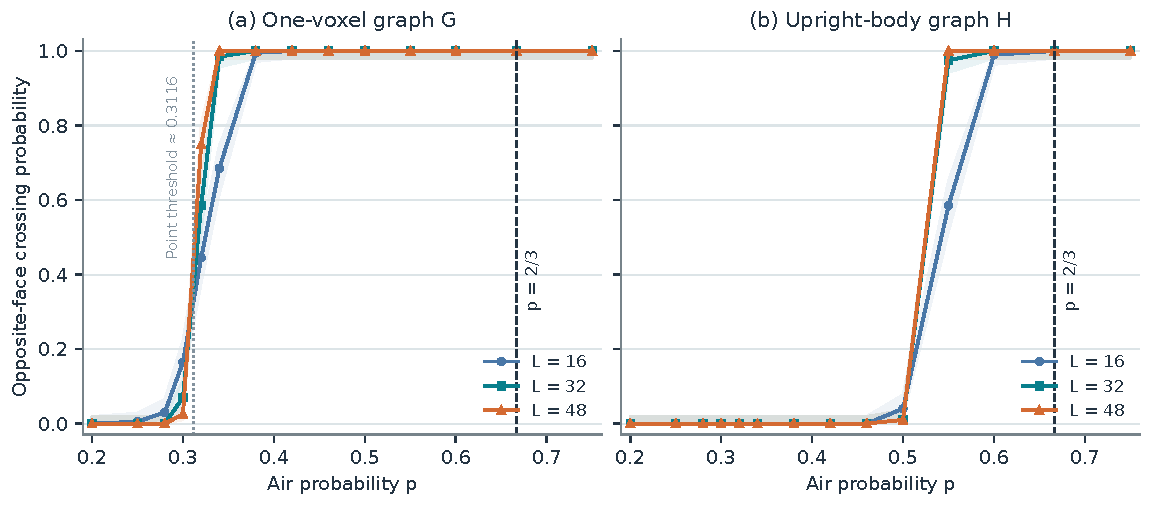
\includegraphics[width=\linewidth]{figures/02_spanning.pdf}
\caption{Empirical opposite-face crossing probabilities for 200 cubes at each
size and density. Shaded regions are pointwise 95\% Wilson intervals.
The dotted reference in (a) is the published independent-site threshold
\citep{wang2013}; it does not apply directly to the dependent graph in (b).
The dashed line marks the proposed air probability $2/3$.
Lines connect sampled densities for readability.}
\label{fig:spanning}
\end{figure}

\begin{table}[htbp]
\centering
\small
\setlength{\tabcolsep}{5pt}
\begin{tabular}{rlrrrrr}
\toprule
$L$ & Model & Crossings & $\bar g$ (\%) & $\bar q$ (\%) & Mean $T$ & 95th pct.\ $T$\\
\midrule
% BEGIN GENERATED RESULTS
16 & One voxel & 300/300 & 99.68 & 99.18 & 1.248 & 1.400 \\
16 & Upright body & 300/300 & 95.31 & 89.92 & 1.710 & 2.067 \\
32 & One voxel & 300/300 & 99.78 & 99.39 & 1.226 & 1.290 \\
32 & Upright body & 300/300 & 96.96 & 92.84 & 1.662 & 1.840 \\
64 & One voxel & 300/300 & 99.82 & 99.45 & 1.207 & 1.238 \\
64 & Upright body & 300/300 & 97.55 & 94.14 & 1.604 & 1.698 \\
% END GENERATED RESULTS
\bottomrule
\end{tabular}
\caption{Focused experiment at $p=2/3$, with 300 independently generated cubes
per size and both movement models evaluated on each cube.
$\bar g$ is the mean largest-component fraction; $\bar q$ is the mean fraction
of admissible entries connected to the exit. Route statistics use one random
admissible entry per cube, conditional on success. Successful route sample
counts for $(G,H)$ are $(297,264)$ at $L=16$, $(299,280)$ at $L=32$, and
$(297,285)$ at $L=64$.}
\label{tab:focus}
\end{table}

Every focused cube admits at least one crossing in both models.
Each $300/300$ outcome has a Wilson interval approximately $[.9874,1]$;
the observations indicate high crossing probability without establishing
certainty for every generated cube. The separate $L=48$ sweep sample at
$p=2/3$ likewise yields 200 crossings in each model.

At $L=64$, on average $99.82\%$ of air vertices belong to the largest component
of $G$. For $H$, $97.55\%$ of admissible body anchors belong to its largest
component. Thus most available space is connected at the proposed density,
including under the height constraint.

\begin{figure}[htbp]
\centering
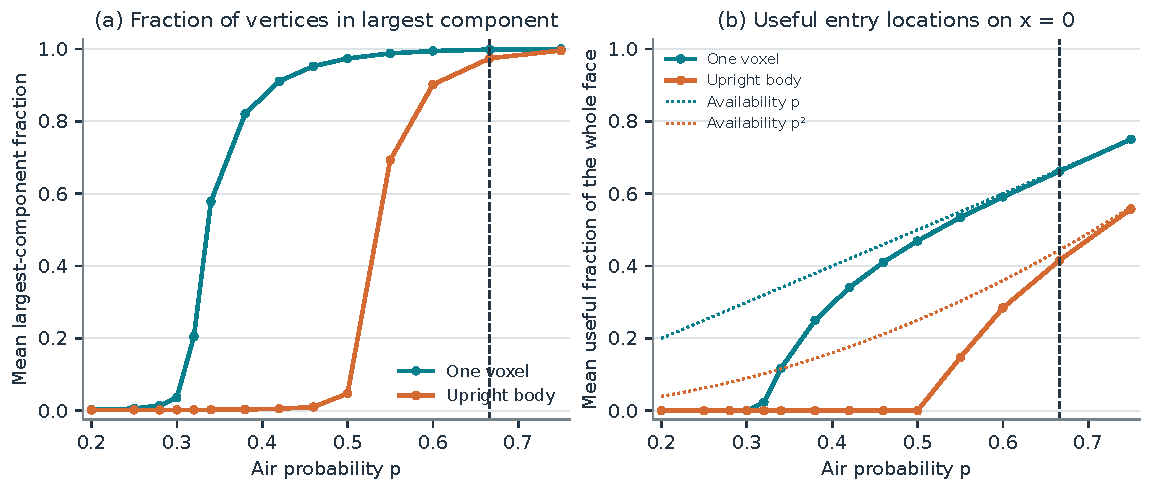
\includegraphics[width=\linewidth]{figures/03_structure.pdf}
\caption{Structure across densities at $L=48$, with 200 cubes per density.
(a) Mean fraction of admissible vertices in the largest component.
(b) Mean fraction of all possible entry locations that connect to the far face.
The dotted curves show expected local availability, $p$ for one voxel and $p^2$
for the upright body. A location can be locally available yet fail to reach
the exit. Bands show approximate pointwise 95\% intervals for the cube means.}
\label{fig:structure}
\end{figure}

\subsection{Finding an entrance and following a route}
At $L=64$, the mean useful fraction of the whole face is $h=0.6633$ for $G$
and $h=0.4188$ for $H$. Among locally admissible entries, the corresponding
mean success fractions are $q=0.9945$ and $q=0.9414$.
The distinction explains two forms of entry search: a candidate location may
be blocked, or it may have enough local clearance while belonging to an
unhelpful component. In these samples, the height constraint affects both.

Figure~\ref{fig:routes} compares the route distributions.
For $L=64$, the mean normalized distance from a random successful entry is
$1.207$ in $G$ and $1.604$ in $H$. The standard deviations are $0.024$ and
$0.062$, and the empirical 95th percentiles are $1.238$ and $1.698$.
The upright model has longer typical detours despite its high crossing
probability. Its mean distance is about $33\%$ larger in this particular
random-entry experiment, although the models sample different admissible
entry sets and are not a same-start path comparison.

\begin{figure}[htbp]
\centering
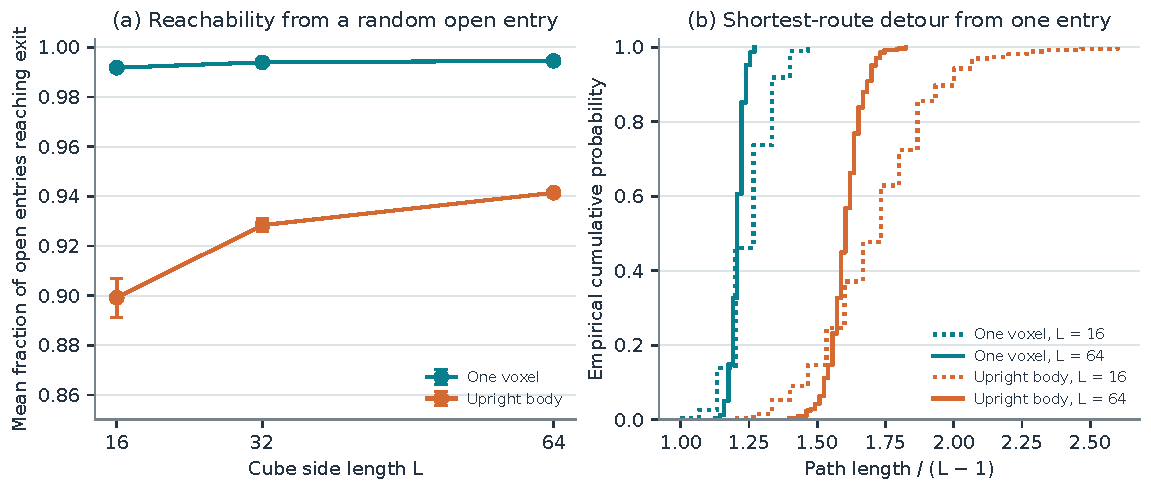
\includegraphics[width=\linewidth]{figures/04_routes.pdf}
\caption{Focused experiment at $p=2/3$.
(a) The exact fraction $q$ is computed per cube and then averaged; error bars
show $1.96$ estimated standard errors. This is not the frequency obtained from
the additional single random entry.
(b) Empirical cumulative distributions of shortest distances from the sampled
successful entries, normalized by $L-1$. Dotted lines show $L=16$ and solid
lines show $L=64$. Failed entries are excluded from these distance distributions
and their counts are reported in Table~\ref{tab:focus}.}
\label{fig:routes}
\end{figure}

With an entry chosen optimally by multi-source BFS, mean normalized crossing
length at $L=64$ falls to $1.111$ in $G$ and $1.422$ in $H$.
An unmarked entrance can therefore change the task even before route selection
inside the volume begins. These graph distances assume full knowledge of the
maze and do not model time spent investigating dead ends.

At the same size, mean cycle rank per admissible vertex is $0.970$ for $G$
and $0.547$ for $H$. The labyrinth contains many independent loops rather than
a single forced corridor. A local observer can face a navigation problem even
when a global shortest-path solver finds a relatively direct crossing.

\subsection{A connected obstacle skeleton can coexist with passages}
The complementary bedrock graph is analyzed in the focused experiment using
the same face-sharing adjacency. Bedrock crosses the cube in $202/300$
realizations at $L=16$, $281/300$ at $L=32$, and $300/300$ at $L=64$.
Because air crosses in all of these realizations, those counts also give the
observed number of simultaneous air-and-bedrock crossings.
At $L=64$, the largest bedrock component contains on average $53.31\%$ of
bedrock voxels, compared with $99.82\%$ of air voxels for the air component.

\begin{figure}[htbp]
\centering
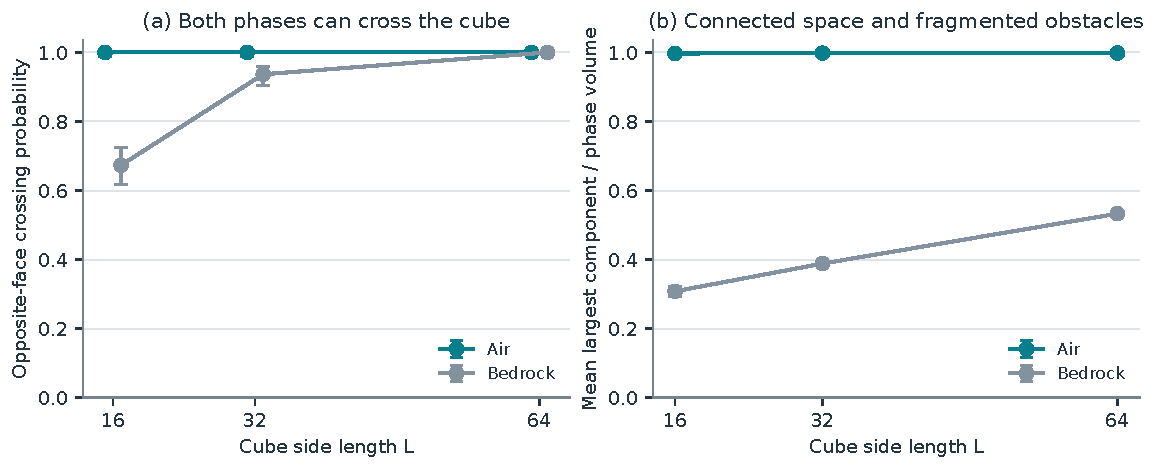
\includegraphics[width=\linewidth]{figures/05_two_phases.pdf}
\caption{Two phases in the same focused cubes at $p=2/3$.
(a) Opposite-face crossing frequencies for air and bedrock, with 95\% Wilson
intervals; horizontal positions are slightly offset for readability.
(b) Mean largest-component size divided by that phase's total voxel count,
with approximate pointwise 95\% intervals for the mean.
Air passages and a spanning obstacle network can occupy the same cube.}
\label{fig:phases}
\end{figure}

This provides a geometric interpretation of the construction: a nearly
connected void winds through a more fragmented but often spanning obstacle
network. The numerical behavior is consistent with the location of both
densities relative to the independent-site threshold. It does not imply that
a bedrock connection forms a separating wall.

\section{Turning the random cube into a playable challenge}
\subsection{An explicit objective}
The simplest experimental objective is to enter through $x=0$, remain inside
the cube, and reach $x=L-1$ without editing any block. Flight-like movement
uses the upright-body graph as a conservative voxel approximation to clearance.
For ground-based play, the generator can remain unchanged while the validator
is replaced by a graph encoding support, jump height, falling, and other
allowed actions. The movement rule should be stated before selecting an
entrance or declaring a level solvable.

The raw volume has many surface openings. A cube without an enforced boundary
also permits an external detour in a surrounding open world. A game must
therefore enforce staying inside, use a suitably placed enclosure, or define
leaving the cube as failure. A physical enclosure changes boundary geometry
and should be included in validation rather than silently added afterward.

\subsection{A crossing-certified generator}
An instance can be generated and certified with the following procedure:
\begin{enumerate}[leftmargin=1.5em,itemsep=3pt]
 \item Sample the cube with air probability $p=2/3$.
 \item Construct the graph corresponding to the chosen movement rules.
 \item Label components and compute the set $U$ of valid entries that reach
 the target face.
 \item If $U$ is empty, draw a new cube. Otherwise choose an entry in $U$,
 select a reachable exit, and retain a path as a solvability certificate.
 \item Apply the intended boundary restrictions and check the final graph.
\end{enumerate}
Rejection sampling produces the original random ensemble conditioned on a
crossing, not an unconditioned Bernoulli sample. Our reported experiments do
not use rejection sampling. If an enclosure or further block edits are made,
rechecking is necessary because the retained certificate may no longer apply.

Entrance selection can also tune the task. Choosing a boundary anchor whose
shortest exit distance lies in a desired range offers a concrete difficulty
control while leaving the interior unchanged. Placing the target inside the
cube, restricting information, or requiring intermediate checkpoints creates
different objectives; each needs its own measurement protocol.

\subsection{What is established and what remains open}
The selected ratio is supported here as a reliably traversable setting for
the two abstract movement models, with substantial connectivity and longer
routes when head clearance is enforced. The study does not optimize $p$ for
fun or difficulty. Lower densities may produce stronger bottlenecks but also
more disconnected instances; a human study would be needed to locate a
preferred tradeoff for a particular player population.

The finite sizes and probability grid do not determine an exact critical
threshold for the upright model. The generator also omits lighting, textures,
visibility, continuous positioning, and action timing. Future work can combine
an actual movement simulator with local-information agents or human trials,
and compare the independent generator with spatially correlated obstacles,
larger passage scales, and exact-composition sampling.

\section{Conclusion}
The 3D Labyrinth turns one weighted random fill into a navigable three-dimensional
object. At two-thirds air, the tested cubes support extensive connected passage
networks, while a two-voxel height requirement introduces additional blocked
entries and longer routes. Finite site percolation explains the construction's
connectivity; configuration-space graphs explain why agent geometry matters.
Together they provide a compact way to generate, analyze, and certify a voxel
exploration challenge originating from a Minecraft livestream.

\smallhead{Origin and computational assistance.}
The concept and WorldEdit prototype are due to Kaoru Aguilera Katayama.
ChatGPT assisted with mathematical exposition, programming, simulation,
figure production, and manuscript preparation. The numerical results are
computer-generated measurements of the stated models, not measurements from
the original Minecraft world.

\smallhead{Data and code availability.}
The paper and its complete reproducibility materials are available in the
project's GitHub repository:
\begin{center}
\url{https://github.com/PolloXDDD/3D-Labyrinth}
\end{center}
The repository includes the compiled PDF, complete \LaTeX{} source,
Bib\TeX{} references, vector figures, the simulation and figure scripts,
the BFS implementation, seeds, metadata, and one row per graph/trial in
\texttt{data/trials.csv}. The exact environment used is recorded in
\texttt{data/metadata.json}. The same materials are provided in the
accompanying source archive.

\begingroup
\interlinepenalty=10000
\bibliographystyle{plainnat}
\bibliography{references}
\endgroup

\appendix
\section{Reproduction and statistical conventions}
After downloading the repository, run the following commands from its root
directory to reproduce the experiments and compile the paper:
\begin{verbatim}
python simulate.py
python figures.py
pdflatex 3d_labyrinth.tex
bibtex 3d_labyrinth
pdflatex 3d_labyrinth.tex
pdflatex 3d_labyrinth.tex
\end{verbatim}
The first command compiles \texttt{bfs.cpp} with a C++17 compiler and executes
the verification checks before generating data. The provided raw data and
figure PDFs also allow the manuscript to be compiled without rerunning
simulations. Python dependencies for the complete pipeline are NumPy, SciPy,
Matplotlib, and pandas. The computation recorded here used Python~3.12.14,
NumPy~2.3.5, SciPy~1.17.0, and GCC~13.3.0 on Linux.

For $k$ successes in $n$ independent cubes, write $\hat s=k/n$ and
$z_{.975}=1.959964$. The Wilson interval used in the figures is
\begin{equation}
 \frac{\hat s+z_{.975}^2/(2n)
 \ \pm\ z_{.975}\sqrt{\hat s(1-\hat s)/n+z_{.975}^2/(4n^2)}}
 {1+z_{.975}^2/n}.
\end{equation}
For a real-valued cube statistic $a_i$, the estimated standard error is
$s_a/\sqrt{n}$, where $s_a$ is the sample standard deviation with denominator
$n-1$. Means of ratios, such as $q$, are computed per cube first and averaged;
they are not replaced by a ratio of pooled counts. Conditional route
percentiles are empirical NumPy/pandas quantiles with linear interpolation.

Random samples are indexed from zero within each experiment. Experiment 1 is
the density sweep; experiment 2 is the focused run; experiment 3 generates only
Figure~\ref{fig:geometry}. Stream 0 generates air. Streams 1 and 2 select a
uniformly random admissible entry for $G$ and $H$, respectively.
The illustrative cube has seed fields $(20261006,3,16,0,0,0)$, and is generated
once without searching for an attractive or successful realization.
Its shortest all-entry path lengths are 16 for $G$ and 22 for $H$.

\end{document}
